%%%%%%%%%%%%%%%%%%%%%%%%%%%%%%%%%%%%%%%%% 
% Stylish Article
% LaTeX Template
% Version 2.1 (1/10/15)
%
% This template has been downloaded from:
% http://www.LaTeXTemplates.com
%
% Original author:
% Mathias Legrand (legrand.mathias@gmail.com) 
% With extensive modifications by:
% Vel (vel@latextemplates.com)
%
% License:
% CC BY-NC-SA 3.0 (http://creativecommons.org/licenses/by-nc-sa/3.0/)
%
%%%%%%%%%%%%%%%%%%%%%%%%%%%%%%%%%%%%%%%%%

%----------------------------------------------------------------------------------------
%	PACKAGES AND OTHER DOCUMENT CONFIGURATIONS
%----------------------------------------------------------------------------------------

\documentclass[fleqn,10pt]{SelfArx}
\usepackage[backend=biber]{biblatex}
\addbibresource{references.bib}
\usepackage[english]{babel}
\usepackage{graphicx}
\graphicspath{ {./imgs/} }
\usepackage[ruled,vlined]{algorithm2e}
\usepackage{xcolor,colortbl}
\definecolor{orange}{rgb}{1,0.647,0}
\usepackage{multirow}


%----------------------------------------------------------------------------------------
%	COLUMNS
%----------------------------------------------------------------------------------------

\setlength{\columnsep}{0.55cm} % Distance between the two columns
\setlength{\fboxrule}{0.5pt} % Width of the border around the abstract

%----------------------------------------------------------------------------------------
%	COLORS
%----------------------------------------------------------------------------------------

\definecolor{color1}{RGB}{0,0,90} % Color of the article title and sections
\definecolor{color2}{RGB}{0,20,20} % Color of the boxes behind the abstract and headings

%----------------------------------------------------------------------------------------
%	HYPERLINKS
%----------------------------------------------------------------------------------------

\usepackage{hyperref} % Required for hyperlinks
\hypersetup{hidelinks,colorlinks,breaklinks=true,urlcolor=color2,citecolor=color1,linkcolor=color1,bookmarksopen=false,pdftitle={Title},pdfauthor={Author}}

%----------------------------------------------------------------------------------------
%	ARTICLE INFORMATION
%----------------------------------------------------------------------------------------

\JournalInfo{Università degli Studi di Milano Bicocca - DISCO}
\Archive{a.a. 2019/20}

\PaperTitle{Amazon Kindle Store Reviews}

\Authors{
  Federico Moiraghi [799735] -
  Pranav Kasela [846965] -
  Roberto Berlucchi [847939]
}

\Keywords{}
\newcommand{\keywordname}{Keywords}

%----------------------------------------------------------------------------------------
%	ABSTRACT
%----------------------------------------------------------------------------------------

\Abstract{
  The present Project is composed by three parts: in the first a model is provided to predict if the buyer of a e-book on Amazon's Kindle Store liked it or not according to the text of the comment; in the second part a recommender system is used to make suggestions about other e-books; in a third part an unsupervised algorithm is used to understand semantics of text, clustering reviews according to their topic.
  All the work is done with both efficiency and effectiveness in mind, providing a valid and scalable solution to all tasks.
}

%----------------------------------------------------------------------------------------

\begin{document}

\flushbottom % Makes all text pages the same height

\maketitle
\tableofcontents
\newpage

\thispagestyle{empty} % Removes page numbering from the first page

%----------------------------------------------------------------------------------------
%	ARTICLE CONTENTS
%----------------------------------------------------------------------------------------

\section*{Introduction}
\addcontentsline{toc}{section}{Introduction}

The present Project is divided into several parts, starting from the same corpus (Amazon's Kindle Store reviews\footnote{\url{https://nijianmo.github.io/amazon/index.html}}), with different purposes.
In the first part, the aim is to provide a good supervised model to predict if a user liked the book or not according to his or her review.
In a second part a collaborative filter will be implemented to provide suggestions to the users according to their preferences.
In the last part, two unsupervised algorithms are tested to clusterize reviews in similar groups: without a ground truth, a semantic analysis of the process is necessary to interpret results.

The entire Project\footnote{Original code is available on GitHub at the link \url{https://github.com/moiraghif/Amazon-Rating-Prediction}} is made using Apache Hadoop\footnote{\url{https://hadoop.apache.org/}} (for data pre-processing) and Apache Spark\footnote{\url{https://spark.apache.org/}} (for the analysis) and is distributed as a Docker image through DockHub\footnote{\url{pkasela/amazon_review_hadoop_spark}}.
The use of a Big Data framework is required by the huge quantity of texts, hardly analyzable by a single machine without taking some precaution: this Project aims not only to provide a valid approach to all the tasks but also to propose a scalable and efficient way to solve them.
Distribution through Docker is considered necessary to simplify installation of dependencies: providing a virtual Operating System (in the specific case, Linux Ubuntu 18.04) with all programs already installed and configured is useful to focus the attention on the \textit{Natural Language Processing} (NLP) pipeline instead of building the environment.\newline
Another reason to use Apache Hadoop and Spark is their ability to parallelize computations to any number of cores or machines supplied, using Scala or Python notebook as usual, in a transparent way to the user.
In particular for this Project Hadoop 3 and Spark 3 are used: those versions are still in a beta phase of development, but have better performance and new functionality than precedent versions.
Data is always kept on the HDFS partition of Hadoop to maximize Spark's performances (in this way data is already partitioned into small chunks).
\begin{figure}[!h]
    \centering
    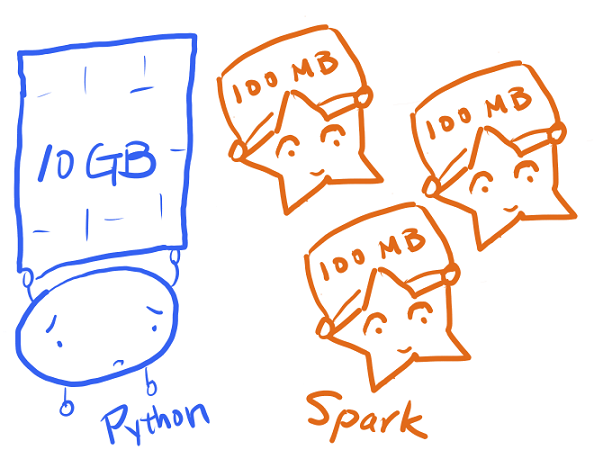
\includegraphics[width=7cm, height=3cm]{pyspark-work.png}
    \caption{How spark manages memory in a more efficient way than Python while managing Big Data and large files in general.}
\end{figure}

Kindle Store corpus is chosen to avoid problems that physical products reviews have in common: a lot of reviews do not focus on the product itself but stress how it was delivered.
Another reason to limit the analysis to the Kindle Store corpus is the fact that its size on disk does not require a cluster (the entire Amazon corpus weights about \verb|700Gb|) but can be processed by a single machine in a reasonable time.

\section{Preprocessing and Data Cleaning}
As the dataset is composed by real reviews from Amazon's Kindle Store, the cleaning part is fundamental to reach good performance on all tasks.
The file is in \verb|.json| format and contains approximately $5 \cdot 10^6$ documents ($5,722,988$ reviews of $493,859$ products) coming from Amazon U.S.A. Kindle Store in a period starting from May 1996 to October 2018.
For each document some recordings are reported, such as ID of the product, of the reviewer, time-stamp (in seconds from epoch), text, rating (number of stars from 1 up to 5) and votes of the review (given by other users).
Fields of interest are selected using a series of regular expression (regex) to parse the \verb|.json| string, instead of the official Python's \verb|json| library, obtaining a $20\%$ gain in speed. \newline

Reviews are written for the most in English, but a small fraction (approximately $5\%$) is composed by texts written in other languages (for the most Spanish or French) or contains just emoticons.
For the purpose of this Project, those reviews are just ignored to avoid the additional complexity caused by the multilingual case.
\verb|CLD-2|\cite{cld2} library is used to filter reviews by language, removing those that are not in English or do not contain text: it uses a Naïve Bayesian Classifier, based (for English) on sequences of four consecutive character, to predict language.
This library is selected among others due to its high speed in managing the quantity of data used in the Project: a comparison made by authors shows that it is more than 200 times faster than Google's \verb|langdetect| and achieves comparable performances in terms of accuracy\cite[6]{cld2}: \newline
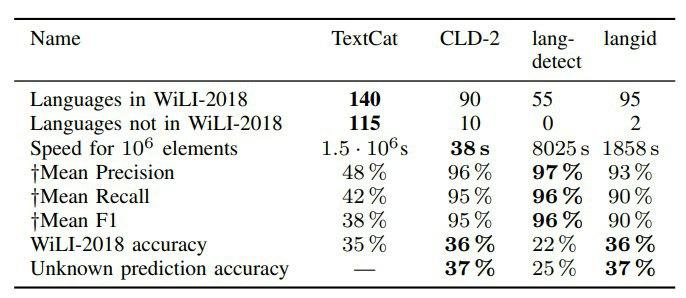
\includegraphics[width=\linewidth]{languages}

After this first phase of cleaning, data is stored in a structured form on the Hadoop file-system (HDFS) and is parsed by a series of regular expression to make it more clean:
\begin{itemize}[noitemsep]
    \item HTML tags and URLs are removed;
    \item punctuation is normalized (e.g. four or more consecutive points are reduced to three);
    \item contractions are re-written in extended form;
    \item particular constructions are re-written in simplified form (e.g. ``have to'' $\rightarrow$ ``must'', ``is going to'' $\rightarrow$ ``will'');
    \item domain-specific terms are simplified (e.g. ``ebook'' $\rightarrow$ ``book'', all Amazon's offers becomes ``Amazon'', all Kindle e-book readers becomes ``kindle'');
    \item numbers are re-written according to their semantics (when easily understandable by the context) or removed (e.g. all prices becomes ``money'');
    \item modal verbs are lemmatized;
    \item words with emphatic repetition of a letter are normalized;
    \item remaining contractions or words composed by a single letter are removed;
    \item punctuation is removed.
\end{itemize}
After this pipeline, the text is processed by a SpaCy\footnote{\url{https://spacy.io/}} model that tokenize sentences and words within each sentence (using a \textit{Deep Learning} approach); each word is then either stemmatized by Porter's Stemmer (second version) offered by NLTK\footnote{\url{http://www.nltk.org/}} or removed if it is a \textit{stopwords}.
Stopwords are taken from NLTK's English list, from which negations and some prepositions are removed, and with the addition of some domain-specific words (such as ``book'' or ``author''). \newline

The entire process, composed by two \textit{only-mapping} jobs, takes one hour and half on a single machine, due to high efficiency provided by HDFS' parallel distribution of the work.
After this process, data is rewritten on the HDFS in a more clean format and is ready to be analyzed.

\newpage
\part{Classification}

\section{Multi-label Classification}
The first task is to predict the vote given by a user according only on the text of the review: while target labels are the number of stars from 1 to 5, input features will be extracted to encode documents in a vectorial space.

\subsection{Exploratory Analysis}
Ratings are not distributed equally: figure \ref{fig:rate_dist} shows that more than half of the reviews gave five stars; and, with the exception of the ``2 stars'' class, lower is the vote, less frequent it is.
\begin{figure}[!h]
    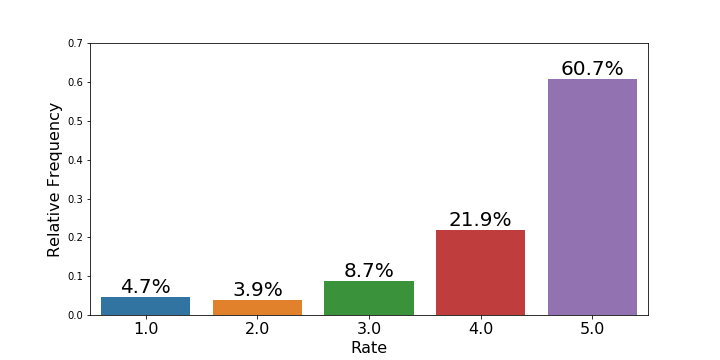
\includegraphics[width=\linewidth]{rate_dist.png}
    \caption{Distribution of review votes (measured in stars).}
    \label{fig:rate_dist}
\end{figure}

To achieve good results, $f_1$ measure is used as performance index instead of \textit{accuracy}, and the model is optimized through a basic grid-search to find a configuration of hyper-parameters that generalize well on the task.

\subsection{Pipeline}
All analysis is made using Apache Spark, reading data directly from HDFS; then a Linear Support Vector Classifier (Liner SVC) is trained to predict classes in a one-vs-all manner: five models will be trained, each one to predict if a document belongs to its class or not.
Six combinations of hyper-parameters are tried in order to get better performance: each combination is tested using 3-folds cross validation to estimate its score.
Then the model with best average score is selected and analyzed in details.
The pipeline is the following:
\begin{itemize}[noitemsep]
\item clean text is tokenized with a simple regex-tokenizer;
\item $n$-grams are extracted;
\item \textit{Tf-Idf} matrix is calculated (\textit{Idf} values are trained only on the \textit{train set}), removing columns with less than 5 occurrences (considered \textit{noise} according to Zipf's Law);
\item \textit{Tf-Idf} values are used to train a one-vs-all SVC model (using only the \textit{train set});
\item $f_1$ is computed on the \textit{validation set}.
\end{itemize}
The grid-search tries to maximize $f_1$ score changing size of $n$-grams and regularization parameter of the machine-learning model; the entire process lasts for about four hours.

\subsection{Results and Interpretation}
\begin{figure}[!h]
  \center
  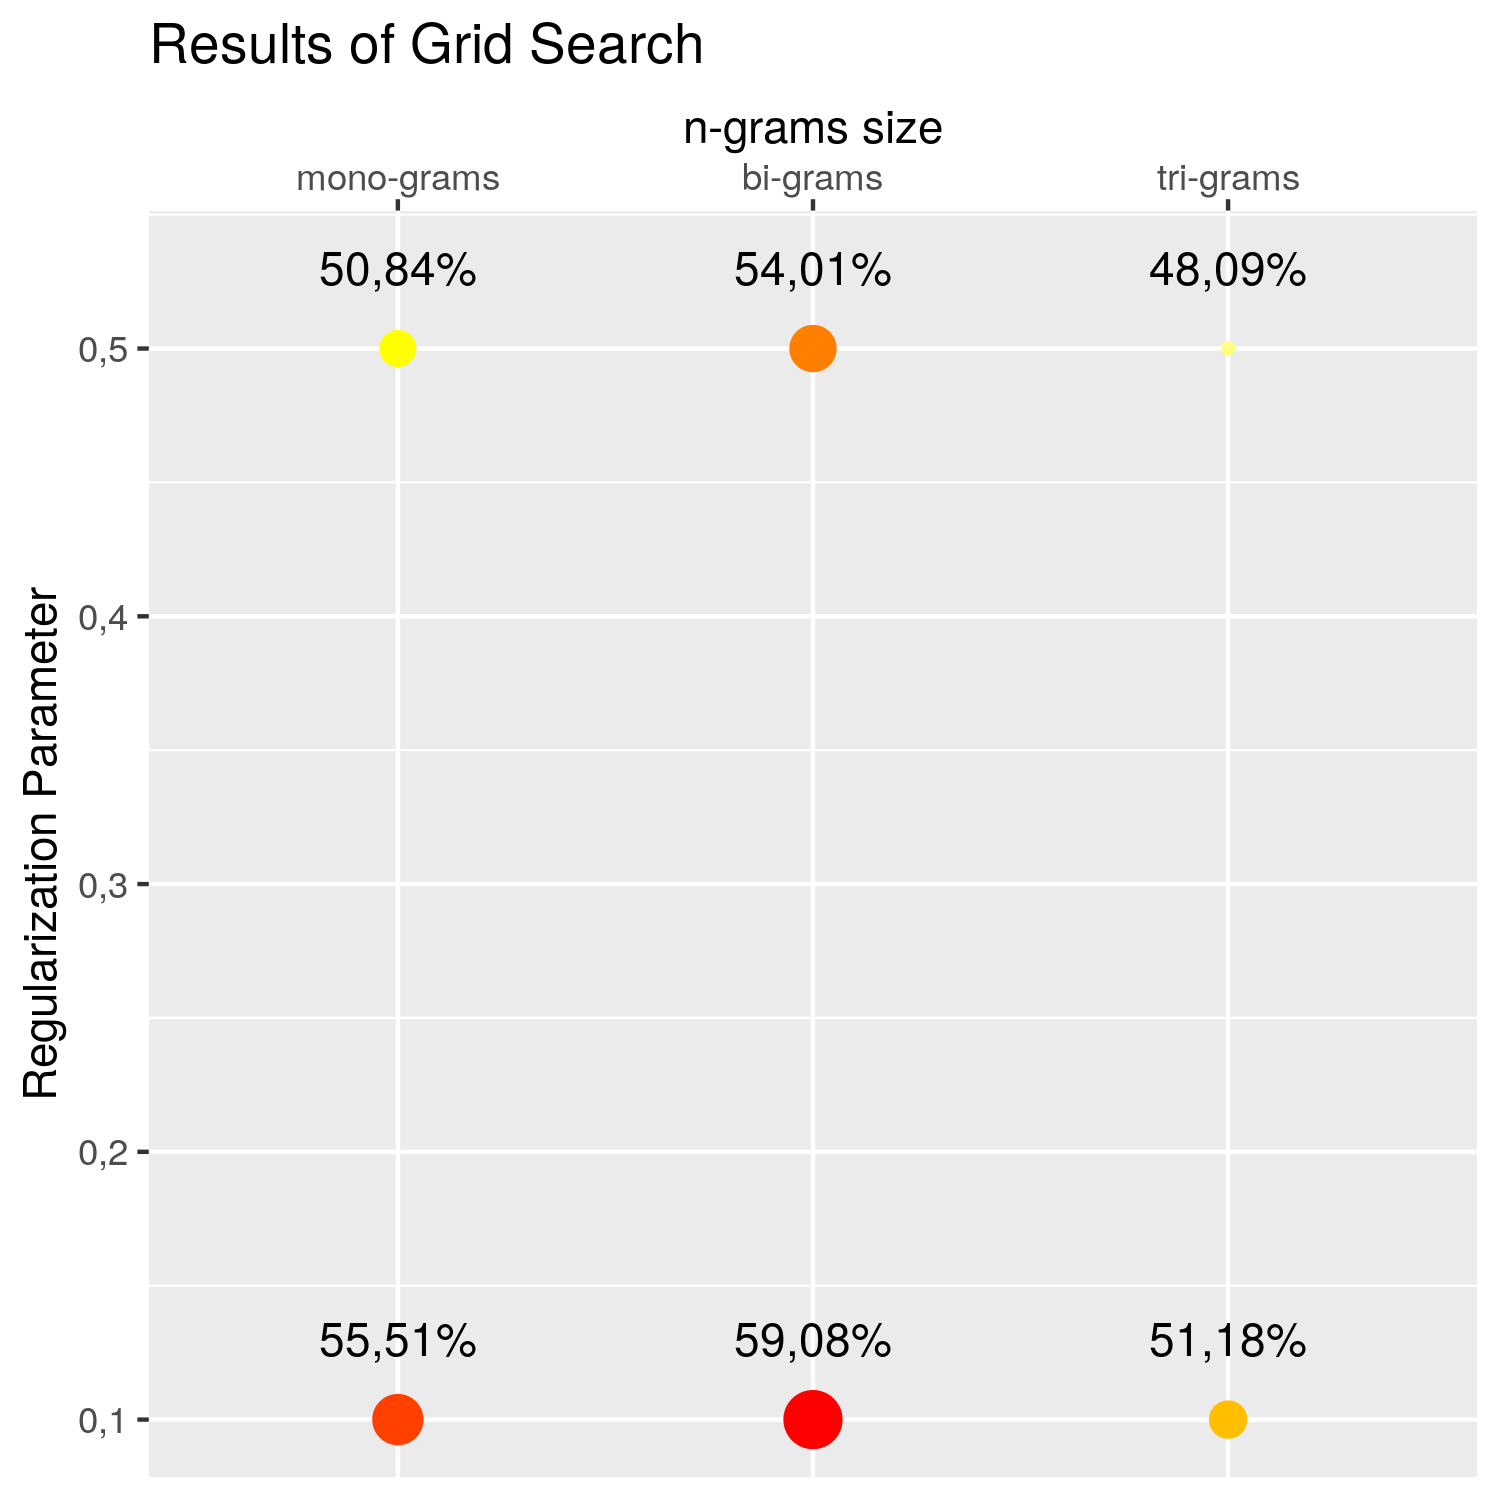
\includegraphics[width=0.8\linewidth]{multi_class_grid_search.png}
  \caption{$f_1$ of the model with various combinations of hyper-parameters.}
  \label{fig:grid_search_multilabel}
\end{figure}

As shown in figure \ref{fig:grid_search_multilabel}, using an SVC classifier, results depends both on Regularization parameter and $n$-gram size, with best results obtained with bi-grams: they can represent simple syntactic constructions (such as ``name + surname'') but without adding an high number of dimensions to the tf-idf matrix.
Tri-grams on the other hand catch more complex constructions but dimensions of the tf-idf matrix is too big for the quantity of data used in this Project.

\begin{figure}[!h]
  \center
  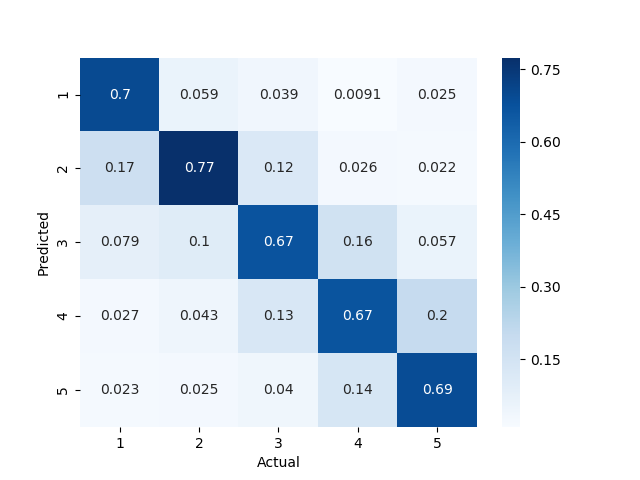
\includegraphics[width=0.9\linewidth]{confusionMatrix_prec.png}
  \caption{Confusion-matrix (normalized by the support) of the multi-label classification with the best configuration.}
  \label{fig:conf_matrix_multilabel}
\end{figure}

Analyzing the regularization parameter, it is clear that reviews are linearly-separable using a tf-idf encoding: best results are obtained with a low value of this parameter.

Results of classification are shown in Figure \ref{fig:conf_matrix_multilabel}: the confusion matrix shows that most reviews are well classified, and most errors occurs between two consecutive labels, although the model does not known that, semantically, are sorted.

\section{Binary Classification}
To improve classification performance, the task is simplified into a binary classification: the model does not predict how much the book has been liked by the reader but just if he or she liked the book.
Target variable is a binary transformation of the number of stars of the review: if the user gave four of five stars to the book, it is considered ``liked''; on the other hand, if the user gave three or less stars, he or she does ``not like'' the book.

\subsection{Exploratory Analysis}
Original ratings given by users are not distributed equally: the two positive classes are the most frequent ones, with a relative frequency of more than $80\%$; but, having $5,473,878$ documents, this percentage is not considered problematic.
In fact, a weighted $f_1$ was used in this case being much more informative for both classes: after a simple optimization pipeline, the resulting model should not be influenced by the unbalance of classes.

\subsection{Classification Pipeline}
The pipeline is identical to the multi-label case, but for the binarization of target variable and the use of a simple logistic regression model instead of one-vs-all SVC.
This is justified by the fact that better performance are achieved by SVC with low regularization parameter, so a linear model should be sufficient to achieve acceptable results, saving training time.
Parameters of search for the grid-search optimization are the size of $n$-grams (starting from 1 up to 3) and the learning rate of the logistic regression (that is computed iteratively for optimization).
The entire process lasts for about two hours: it is clear that using a logistic model is far more efficient (in terms of computational time) compared to the previous one.

\subsection{Results and Interpretation}
\begin{figure}[!h]
  \center
  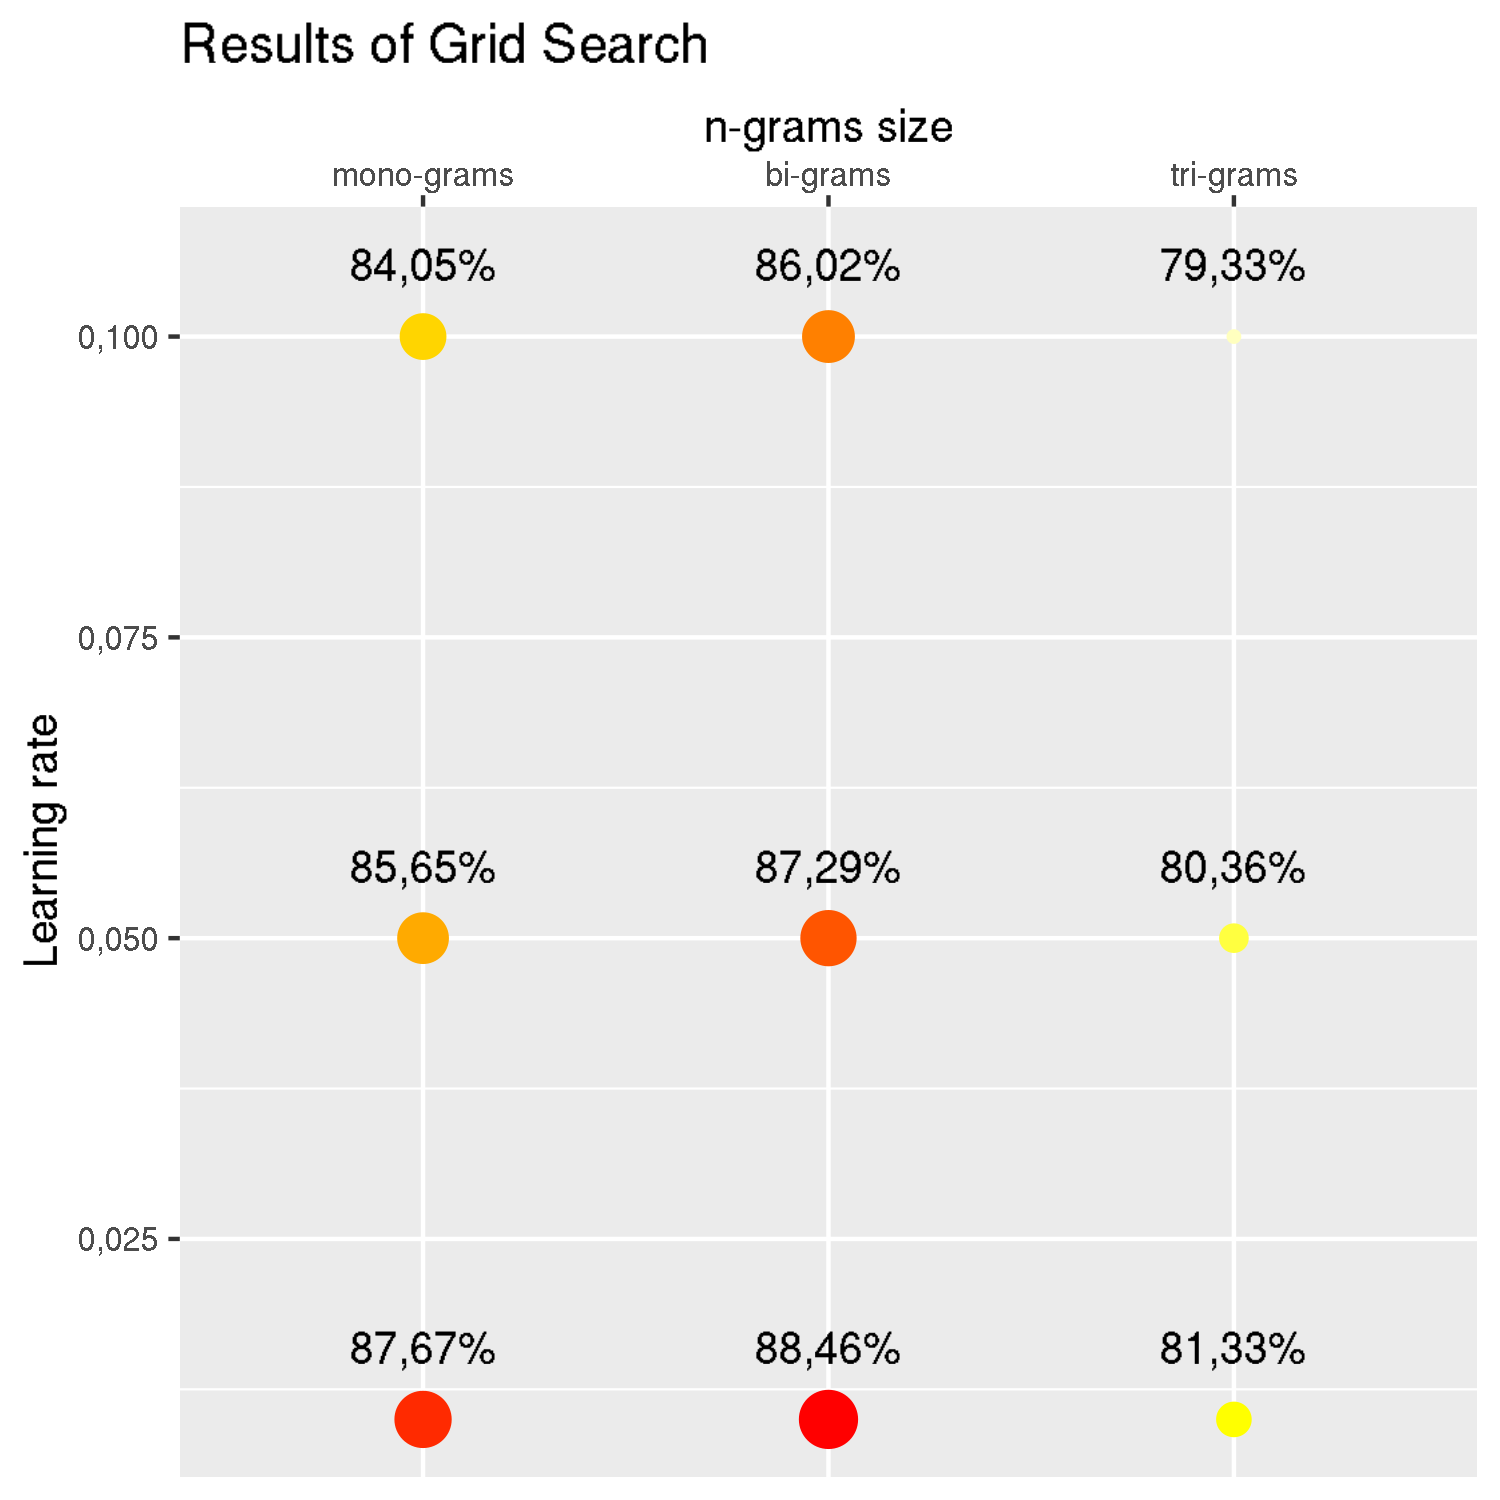
\includegraphics[width=0.8\linewidth]{binary_class_grid_search.png}
  \caption{Results of grid search of binary classification. Values represent the weighted $f_1$ of the model using the corresponding configuration.}
  \label{fig:grid_search_binary}
\end{figure}
As shown in figure \ref{fig:grid_search_binary}, the best configuration found in the process is obtained using \textit{bi-grams} with a low \textit{learning rate}.
Poor performances yielded by the use of \textit{tri-grams} can be again justified by the insufficient quantity of data: resulting matrix is very high-dimensional, so the risk of \textit{overfitting} the \textit{train set} is very high.
From a NLP perspective, results have to be interpreted in the same way as previous ones: \textit{bi-grams} catch some semantics, \textit{tri-grams} catch even more but their use produce an overfitting of the train set.

The $f_1$ on the rare class (not-liked) is $0.69$, with precision$=0.85$, recall$=0.58$, and an overall accuracy of $0.91$

\subsection{Possible Improvements}
Due to higher performance of \textit{bi-grams} instead of \textit{mono-grams}, one strategy to improve results consists of using a simple Ontology to support the tokenization of texts, to replace names of authors, characters or titles with the corresponding URI; or in alternative, an Entity Recognition algorithm can be used to obtain better tokens.
They are both very sophisticated ways to normalize names and titles, but their implementation is very expensive (in terms of time and money) and their use can be excessive resource-demanding.

\subsection{Possible Uses of the Model}
Using texts written in natural language in a informal context, the Model should generalize well on texts taken from other social media (such as Facebook or Twitter).
This model therefore can be tested on social media platforms to make market research or to integrate data from different sources in a Recommending System.


\section{Sentiment Polarity}
To prove the correlation between review text and rate, a pre-trained model\footnote{Included in Python TextBlob library, see documentation at: \url{https://textblob.readthedocs.io/en/dev/quickstart.html\#sentiment-analysis}.} is used to assign a score between $-1$ and $+1$ to each review.
Raw text is used for this task, since even stop words can change the polarity calculated by the TextBlob library.
It can be useful to see how much the sentiment, which is considered as an ordinal value, is correlated to the rate: it may be an external regressor, together with the tf-idf, for future improvements.

The correlation between the two variables is $\varrho = 0.37$: sentiment extracted from text can be added to the previous model for the vote prediction. 
It is clear that, greater is the average Sentiment Polarity, better the rating is going to be for a product.
This can be also seen by taking the average sentiment for number of star:
\begin{figure}[!h]
    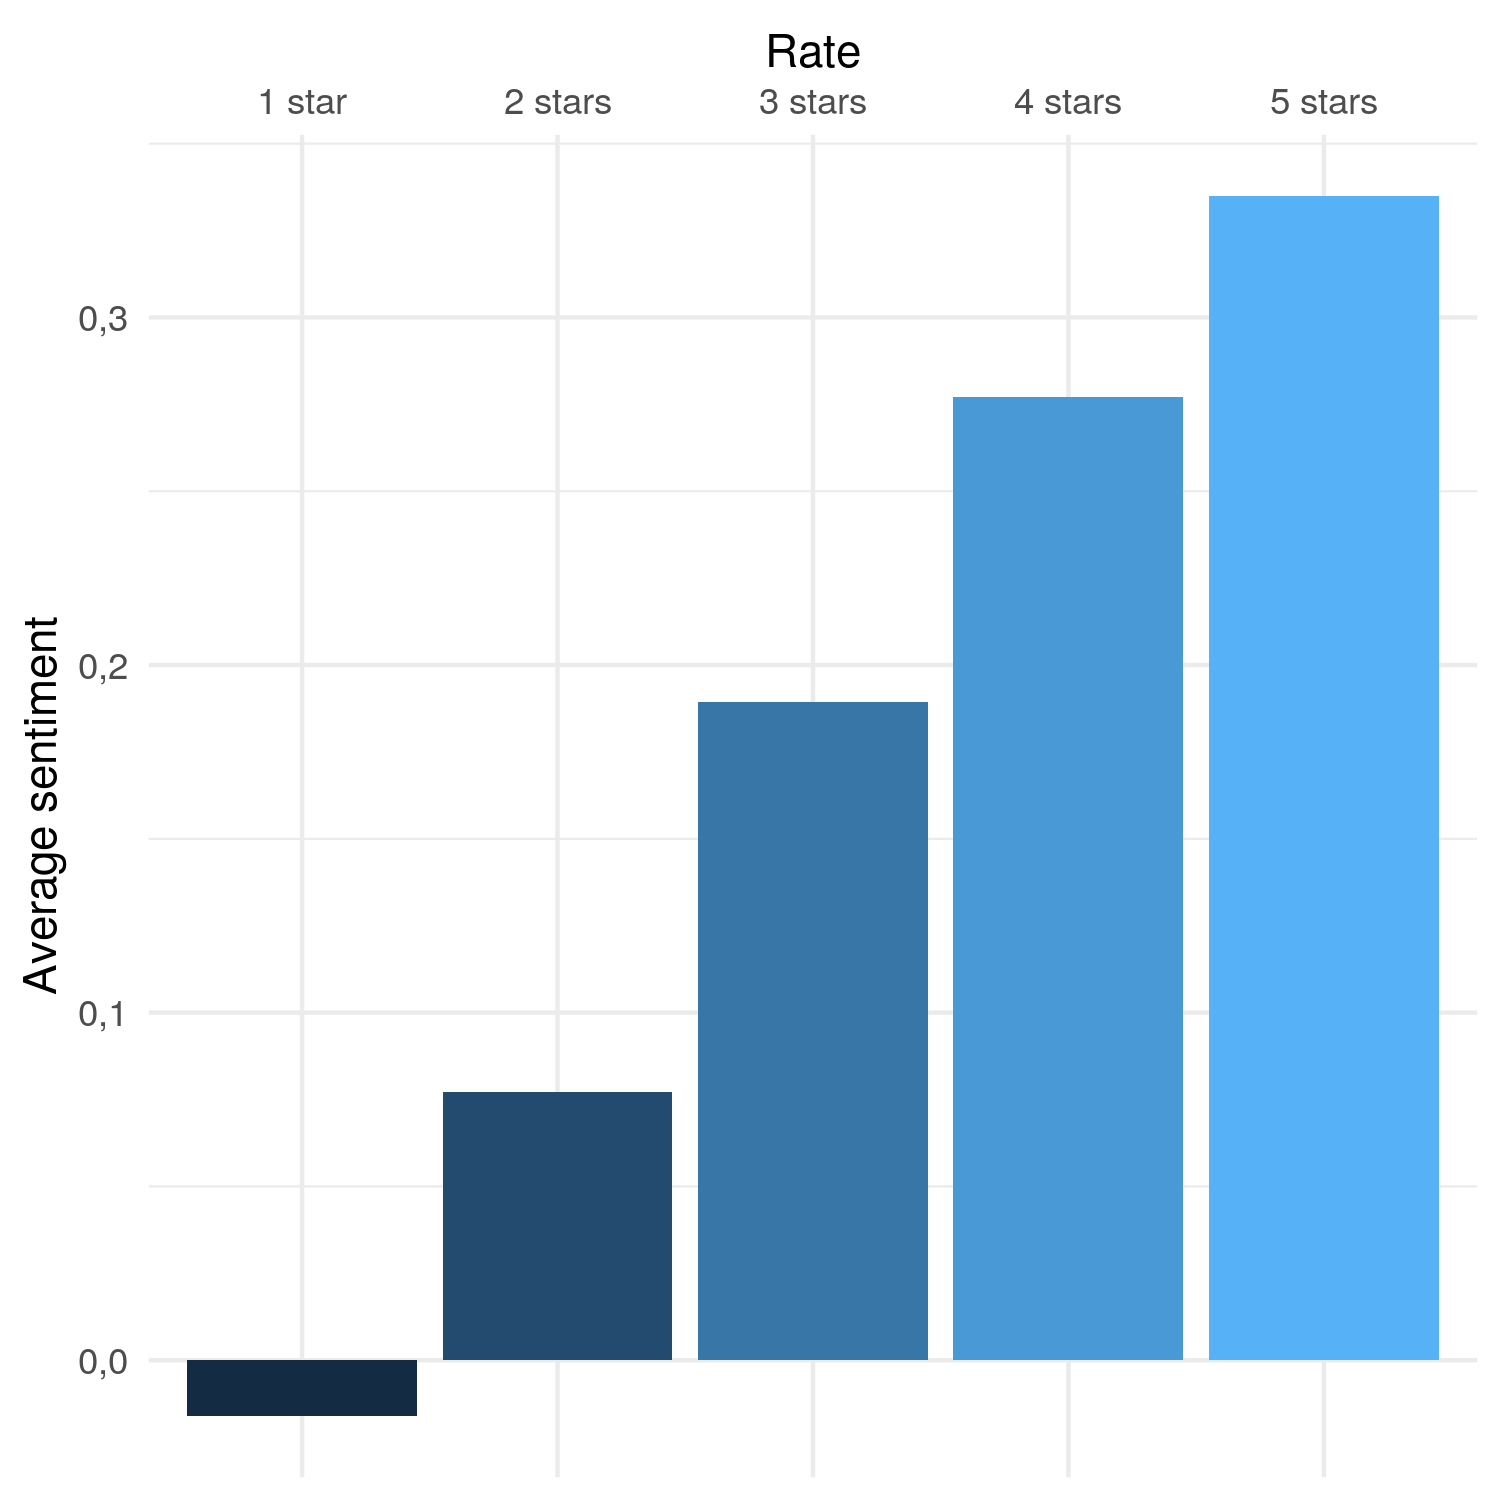
\includegraphics[width=\linewidth]{sentiment.png}
    \caption{Average Sentiment Polarity for each review star.}
    \label{fig:sentiment}
\end{figure}

\newpage
\part{Recommender System}
\section{Collaborative Filtering}
The algorithm used to implement the collaborative filtering is ALS (\textit{Alternating Least Squares}), included in Apache Spark.
To optimize the process, Apache Spark does not store User-Product matrix $R$ in a direct way but it decompose it into two matrix $U$ and $V$ (such that $R = U \times V$), estimated with an iterative process.
The iteration starts with random guess of the $U$ and $V$ matrix and alternatively use the least squares to reach the approximation of the two matrices.
This method is extremely efficient, since the SVD (like any other way to factorize a matrix) has a quadratic computational cost, while the ALS, at the cost of some precision, is able to do it in a limited number of iterations and it works well also with implicit ratings, although is not the case.
\begin{figure}[!h]
    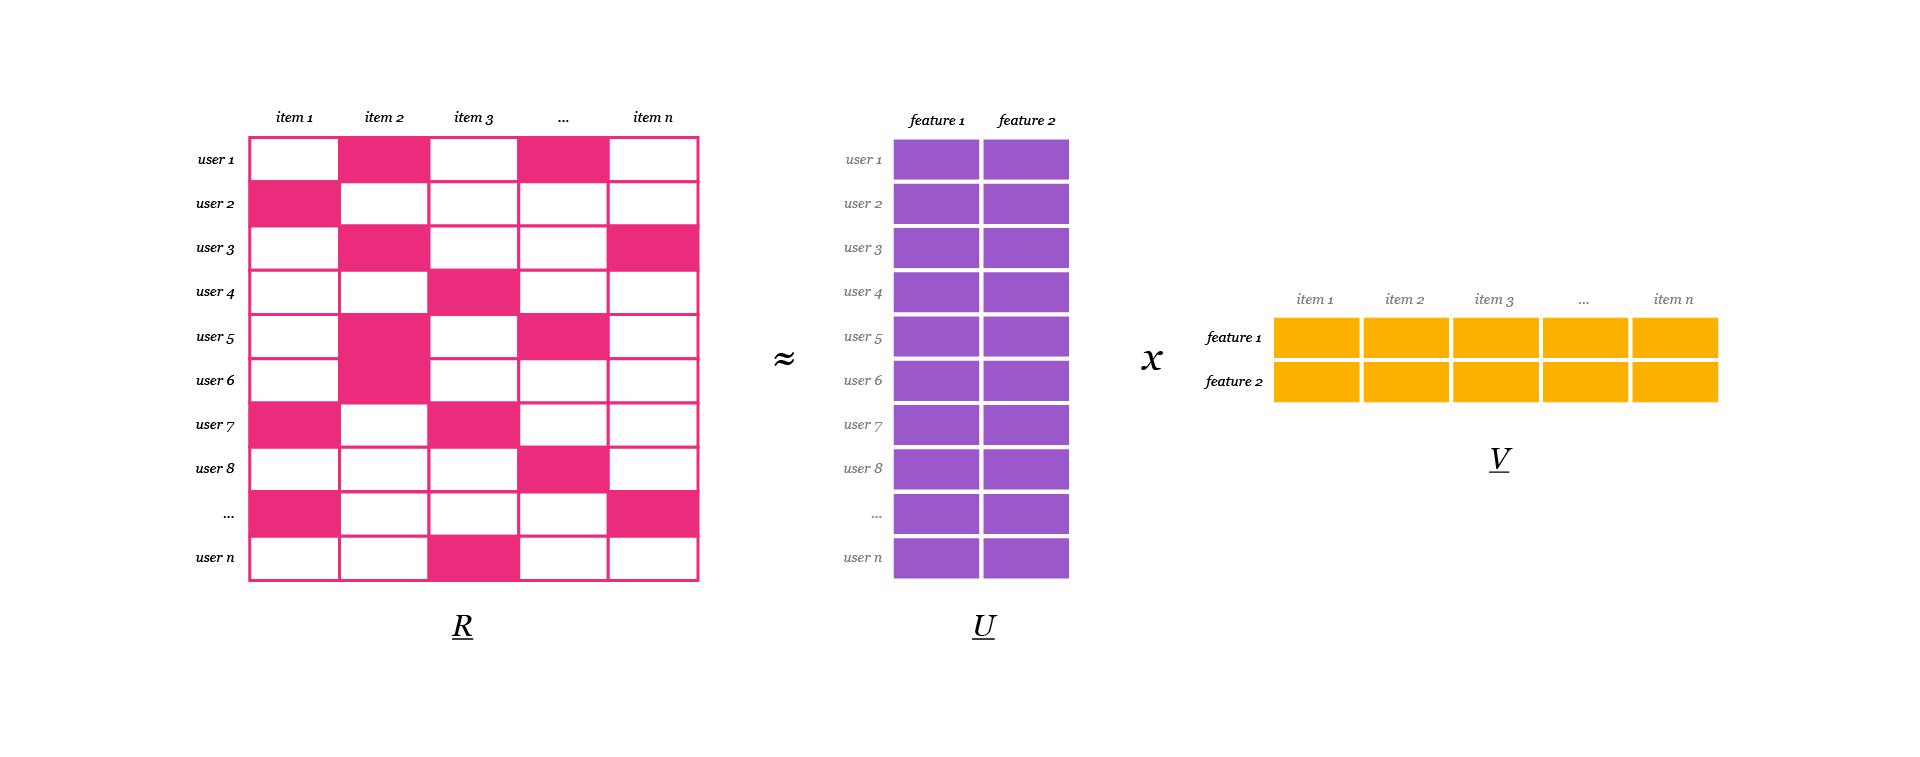
\includegraphics[width=\linewidth]{als.png}
    \caption{Representation of the ALS factorization.}
    \label{fig:als}
\end{figure}

Once factorized the $R$ matrix, the $V$ matrix is used to find items that are similar (using the dot product) and to make the recommendation for the $i$-th user is computed as: $score = U_i \times V^T$.
So only the UserID, Product and the rating given to the product by the user is needed.

The hyper-paramters of this models are the regularization parameter $\lambda$, the number of iterations and the rank (number of features).
A grid-search optimization (using a 3-folds cross validation) is used to find best configuration of hyper-parameters, using RMSE (\textit{Root Mean Squared Error}) as performance index (trying to minimize it).
Relevance score is the rating itself, as number between 1 and 5.

The time efficiency can be seen also by the fact that it takes around only one minute to fit the model and one minute to evaluate it in each fold of the cross-validation.

\subsection{Results}
\begin{table}[!h]
    \centering
     \begin{tabular}{|c|c|c|c|}
          \hline
          $\lambda$ & maxIter & rank & RMSE\\
          \hline
          0.05 & 10 & 5  & 0.9045\\
          0.05 & 10 & 10 & 0.9294\\
          0.05 & 10 & 20 & 0.9379\\
          0.05 & 15 & 5  & 0.8934\\
          0.05 & 15 & 10 & 0.9094\\
          0.05 & 15 & 20 & 0.9058\\
          0.1  & 10 & 5  & 0.8318\\
          0.1  & 10 & 10 & 0.8332\\
          0.1  & 10 & 20 & 0.8286\\
          0.1  & 15 & 5  & 0.8262\\
          0.1  & 15 & 10 & 0.8242\\
          \rowcolor{orange} 
          0.1  & 15 & 20 & 0.8171\\
          \hline
     \end{tabular}
    \caption{grid-search results for ALS.}
    \label{tab:als_grid}
\end{table}

Best configuration (highlighted in the Table \ref{tab:als_grid}) obtains an RMSE of $0.8171$. 
The model improves as the number of iteration grows but the improvement is really small, and risk of overfitting will increase: using a low number of iteration can yield a model with lower performance but that generalize better.

\subsection{Possible Uses of the Model}
Being a Recommender system, using this model it is possible to provide users with suggestions about not-yet-reed e-books.
Being fast to train and easily scalable, this model can be re-trained regularly, going behind the assumption that user's tastes do not change.

\newpage
\part{Clustering}
\section{$K$-means}
Data is also clustered using the processed dataset (without stopwords, stemmatized and normalized): $n$-grams are extracted from text reviews, are used to encode the document with tf-idf, and finally a $k$-means algorithm (with Euclidean distance) is used to group them in clusters

\subsection{Other $k$-means variants}
$K$-means (using the classic Lloyd algorithm) takes $k$ random centers and iterates until convergence.
It is a very simple and scalable algorithm but it has a few shortcomings:
\begin{itemize}[noitemsep]
\item it takes many iteration (on average) to converge;
\item it is very sensitive to the initial points;
\item random points can be initiated in the same cluster, and the $k$-means gets stucked in a local optima.
\end{itemize}
Actually getting optimum initial points for the $k$-means is a NP-hard problem, and Llyod method trivializes it: using random sampling trying to solve a NP-hard problem in a constant time, thus degrading $k$-means performance.
An alternative approach, used in this case, is the $k$-means++ algorithm \cite{kmeans++}, which initializes centroids in an intelligent way, here is how it works:

\begin{algorithm}
  \SetAlgoLined
 Choose the first center, $c_1$, uniformly at random from the data set\;
 \For{ $2\leq i \leq k$ } {
    $\forall x$ calculate $d(x)$, the distance between x and the nearest center\;
    Choose $c_i$ to be sampled from the data with probability $\propto d(x)^2$\;
 }
 Proceed with the usual $k$-means algorithm;
 \caption{k-means++}
\end{algorithm}
The $k$-means++ version needs $k$ passes on the data before actally starting the iterative process, and has troubles to scale with large data applications or an high number of centroids. 
There is a variant implemented in Apache Spark and used in this Project: $k$-means$||$\cite{kmeans||}, which basically updates the distribution less frequently, oversampling each point with a larger probability.
This variant is able to scale well through parallelization, and requires less passes on the data in initial phase, yielding similar results.
The initial passes reduces the clustering effort later on, reducing the overall convergence time.
Being initialized in an optimal way, results are generally compared to Lloyd's $k$-means.

To find the optimal number of clusters $k$ and the optimal size $n$ for the $n$-grams, a grid-search is performed with $2\leq k \leq 7$ and $1 \leq n \leq 3$, while trying to maximize the silhouette.
The optimal cluster is with $n=1$ and $k=2$ with a silhouette$=0.78$.

\begin{figure}[!h]
     \centering
     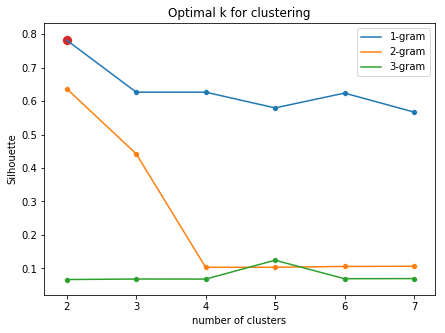
\includegraphics[width=\linewidth, height=5cm]{k_mean_opt.png}
     \caption{Optimal $K$-means and $n$-grams grid-search.}
\end{figure}

Once fixed the number of clusters $k$, the time required for executing the pipeline (Tf, Idf, Clustering and Evaluation) depends only on the $n$-grams size, in particular for $n=1$, the clustering required approximately 20 minutes, while for $n=2$ it required 17 minutes and finally for $n=3$ (which increases a lot the dimensions) required 85 minutes.
Surprisingly the time does not change too much if the number of cluster changes due to parallelization of the process.

\subsection{Results and Interpretation}
The actual number of optimal clusters is lower than expected, moreover the number of elements within groups are surprising: the first cluster has $5,057,795$ elements and the second one only $396,720$.
The two cluster's average rate is very similar, $4.22$ and $4.31$ respectively, so the distinction of the cluster is not given by the negative or positive words.
The most frequent words of the two clusters overlaps: one method to improve the process could be to remove those common words and try again.
This approach might not be the best option since some of these words seem to be important such as: ``story'', ``great'', ``enjoy'' or ``interesting''.

Having poor performance, this approach is abandoned in favour of another type of exploratory technique: \textit{Topic Modeling}.

\section{LDA - Topic Modeling}
The basic hypothesis behind LDA is that a document is made up of a set of arguments, which are characterized by a distribution of words.
The objective of LDA\cite{lda} is to find the latent arguments (topics): analyzing the similarity between the distribution of words in the document, it helps to understand the semantics of the text.
Mathematically it tries to learn:
$$P(\theta, z, w | D, \alpha, \eta)$$
where $\theta$ is a distribution of topics, a $k$-dimensional random Dirichlet variable, $z$ is the number of topics for each document, $w$ is the distribution of words for each topic, $D$ is the corpus, $\alpha$ is the document-topic distribution and $\eta$ is the topic-word distribution.
Only words appearing in at least 30 documents are considered, the number of topics is fixed to 10 and the maximum number of iterations, given the ``poor'' results of $k$-means, was chosen to be 100.

\subsection{Results and interpretation}
The algorithm converges in 3:30 hours and the topics found are:
\begin{table}[!h]
    \resizebox{\columnwidth}{!}{
        \begin{tabular}{|c|c|c|c|c|}
        \hline
        \multicolumn{5}{|c|}{Topic}\\
        \hline
        1            & 2        & 3        & 4         & 5 \\
        \hline
        love         & picture  & love     & life      & town\\ 
        not          & money    & hot      & god       & murder\\
        want         & version  & not      & children  & mate\\ 
        get          &  color   & wait     & help      & find \\
        one          & download & sa       & love      & friend\\ 
        feel         & not      & seri(es) & us        & famili(y)\\ 
        relationship & ship     & sex      & kid       & mysteri(y)\\ 
        man          & print    & one      & live      & love\\ 
        life         & free     & stori(y) & inspir(e) & emma\\ 
        know         & use      & sexi(y)  & stori(y)  & bear\\
        \hline
        \multicolumn{5}{|c|}{Topic}\\
        \hline
        6           & 7         & 8          & 9           & 10 \\
        \hline
        novel       & recip(e)  & money      & seri(es)    & not \\ 
        world       & food      & war        & stori(y)    & money \\
        money       & eat       & busi(y)    & charact(er) & like \\ 
        stori(y)    & diet      & use        & love        & good\\ 
        render      & easi(y)   & histori(y) & enjoy       & no\\ 
        charact(er) & inform    & inform     & not         & time\\ 
        tale        & use       & peopl(e)   & great       & get\\ 
        fiction     & cook      & understand & next        & edit\\ 
        time        & weight    & work       & read        & use\\ 
        one         & healthi(y)& practic    & end         & word\\
        \hline
        \end{tabular}
    }
    \caption{Extracted topics with top 10 words describing it.}
    \label{tab:lda}
\end{table}
  
From the words describing the topics in Table \ref{tab:lda}, in the most cases, the real topics such as genre can be deduced: for example the second topic is about the kindle format of book itself, the third topic is about some erotic/romantic genre, the fifth topic seems to talk about some crime related books, the seventh topic about some cookbooks, the eight topic about some historical genre.
While some topics most probably describes the feeling of the reviewer, the forth one talks about some inspiration in life and god, which can be either a gospel kind of genre or the feeling of the reviewer, the ninth one talks about enjoying and wanting to read some other books.

\subsection{Possible Uses of the Model}
This model can be used to check if an informal text written by a human is about a particular genre of book.
Its use make possible to analyze external sources of information to check which genre is talked in a particular \textit{web community} (such as \textit{sub-reddits} or social network web pages), providing targeted advertising to users.



%----------------------------------------------------------------------------------------
%	REFERENCE LIST
% ----------------------------------------------------------------------------------------
\newpage
\part*{Conclusions}
During the Project different solutions to different tasks have been presented, concerning \textit{Natural Language Processing} on commercial texts about e-books.
Two \textit{machine learning} models have been proposed to segment market according to reading tastes and to predict if the opinion of the reader is good or not about a particular e-book.
In addition, a simple but effective recommender system is analyzed to understand how it works  on a cluster of data in a efficient and scalable way.

\newpage
\nocite{*}
\printbibliography


%----------------------------------------------------------------------------------------

\end{document}
% LocalWords:  recommender
